\documentclass{beamer}
\usetheme{metropolis}

% specifications for presenter mode
%\beamerdefaultoverlayspecification{<+->}
%\setbeamercovered{transparent}

\usepackage[english]{babel}
\usepackage[utf8x]{inputenc}

%\usepackage{coloremoji}
\usepackage{layout}
\usepackage{multirow}
\usepackage{array}
\usepackage{graphicx}
\graphicspath{ {Figs/} }
\usepackage{animate}

\setbeameroption{hide notes}
\setbeamertemplate{note page}[plain]
\usepackage{listings}
\usepackage{datetime}
\usepackage{url}
\usepackage{tcolorbox}
\usepackage{appendixnumberbeamer}

\usepackage{tikz}
\def\checkmark{\tikz\fill[scale=0.4](0,.35) -- (.25,0) -- (1,.7) -- (.25,.15) -- cycle;}

% math shorthand
\usepackage{bm}
\usepackage{amstext}
\usepackage{amsthm}
\usepackage{amsmath}
\usepackage{mathtools}
\newcommand{\R}{\mathbb{R}}
\newcommand{\D}{\mathcal{D}}
\newcommand{\E}{\mathbb{E}}
\newcommand{\I}{\mathbb{I}}
\newcommand{\pr}{\mathbb{P}}
\newcommand{\F}{\mathcal{F}}
\newcommand{\X}{\mathcal{X}}
\newcommand{\M}{\mathcal{M}}
\newcommand{\lik}{\mathcal{L}}

\newtheorem*{assumption*}{\assumptionnumber}
\providecommand{\assumptionnumber}{}
\makeatletter
\newenvironment{assumption}[2]
 {%
  \renewcommand{\assumptionnumber}{Assumption #1: $\mathcal{#2}$}%
  \begin{assumption*}%
  \protected@edef\@currentlabel{#1: $\mathcal{#2}$}%
 }
 {%
  \end{assumption*}
 }
\makeatother

\DeclarePairedDelimiterX{\infdivx}[2]{(}{)}{%
  #1\;\delimsize\|\;#2%
}
\newcommand{\infdiv}{D\infdivx}
\DeclarePairedDelimiter{\norm}{\lVert}{\rVert}
\DeclareMathOperator*{\argmin}{arg\,min}
\DeclareMathOperator*{\argmax}{arg\,max}

% indepndence notation macro
\newcommand\indep{\protect\mathpalette{\protect\independenT}{\perp}}
\def\independenT#1#2{\mathrel{\rlap{$#1#2$}\mkern2mu{#1#2}}}

% Bibliography
\usepackage{natbib}
\bibpunct{(}{)}{,}{a}{}{;}
\usepackage{bibentry}

\title{\normalsize Mediation analysis with stochastic interventions}

\author{\href{https://nimahejazi.org}{Nima Hejazi}\\[-10pt]}

\institute{
  \begin{figure}[!htb]
    \centering
    \begin{minipage}{.65\textwidth}
        Graduate Group in Biostatistics, and \\
        Center for Computational Biology, \\
        University of California, Berkeley \\[6pt]
        
\includegraphics[scale=0.12]{twitter-icon.png}
          \href{https://twitter.com/nshejazi}{nshejazi} \\
        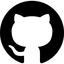
\includegraphics[scale=0.09]{github-icon.png}
          \href{https://github.com/nhejazi}{nhejazi} \\
        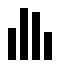
\includegraphics[scale=0.12]{homepage.png}
          \href{https://nimahejazi.org}{nimahejazi.org} \\
        
\includegraphics[scale=0.12]{pdf-icon.png}
        \href{https://bit.ly/2020\_acic\_mediate}{bit.ly/2020\_acic\_mediate} \\
        {\scriptsize joint work with Iv\'an D\'iaz and Mark van der Laan}
    \end{minipage}%
    \begin{minipage}{0.35\textwidth}
      \centering
      
\includegraphics[height=0.80in,width=0.80in]{ucberkeleyseal_874_540.eps}
    \end{minipage}
  \end{figure}
}

\date{\today}

%%%%%%%%%%%%%%%%%%%%%%%%%%%%%%%%%%%%%%%%%%%%%%%%%%%%%%%%%%%%%%%%%%%%%%%%%%%%%%%%

\begin{document}

\begin{frame}[noframenumbering]
  \thispagestyle{empty}
  \titlepage
\end{frame}

%%%%%%%%%%%%%%%%%%%%%%%%%%%%%%%%%%%%%%%%%%%%%%%%%%%%%%%%%%%%%%%%%%%%%%%%%%%%%%%%

\begin{frame}[c]{Stochastic Population Intervention (In)Direct Effects}

\begin{center}
\begin{itemize}
\itemsep2pt
\item Consider observed data $O = (W, A, Z, Y) \sim P_0 \in \mathcal{M}$, with
  no assumptions on nonparametric model $\mathcal{M}$.
\item \cite{diaz2019causal} decompose the total population intervention effect
  (PIE) in terms of a \textit{direct effect (PIDE)} and an \textit{indirect
  effect (PIIE)}:
  \begin{equation*}
    \psi(\delta) = \overbrace{\mathbb{E}\{Y(A_\delta, Z(A_\delta)) -
       Y(A_\delta, Z)\}}^{\text{PIIE}} + \overbrace{\mathbb{E}\{Y(A_\delta, Z)
       - Y(A, Z)\}}^{\text{PIDE}}.
  \end{equation*}
\item The causal parameter $\mathbb{E}\{Y(A_\delta, Z)\}$ is required for
  estimation of the PIIE or PIDE; other components already estimable.
\end{itemize}
\end{center}

\note{
}

\end{frame}

%%%%%%%%%%%%%%%%%%%%%%%%%%%%%%%%%%%%%%%%%%%%%%%%%%%%%%%%%%%%%%%%%%%%%%%%%%%%%%%%

\begin{frame}[c]{Stochastic Population Intervention (In)Direct Effects}

\begin{center}
\begin{itemize}
\itemsep2pt
\item \cite{diaz2019causal} show $\mathbb{E}\{Y(A_\delta, Z)\}$ is identified by
  \begin{equation*}
    \theta(\delta) = \int m(z, a, w)g_{\delta}(a\mid w)p(z,w) d\nu(a,z,w),
  \end{equation*}
  for outcome mechanism $m(z,a,w)$ and post-intervention treatment mechanism
  $g_{\delta}(a\mid w)$.
\item Efficient influence function (EIF) for $\theta(\delta)$ in $\mathcal{M}$
  is given with 3 components $D^Y_{\eta, \delta}(o) + D^A_{\eta, \delta}(o) +
  D^{Z, W}_{\eta, \delta}(o)$, where $\eta$ indexes nuisance parameters.
\end{itemize}
\end{center}

\note{
}

\end{frame}


%%%%%%%%%%%%%%%%%%%%%%%%%%%%%%%%%%%%%%%%%%%%%%%%%%%%%%%%%%%%%%%%%%%%%%%%%%%%%%%%

\begin{frame}[c]{Stochastic Population Intervention (In)Direct Effects}

\begin{center}
\begin{itemize}
\itemsep2pt
\item For simplicity, let $A \in \{0, 1\}$ and consider incremental propensity
  score interventions \citep{kennedy2017nonparametric}, EIF given as
  \vspace{-0.5em}
  \begin{align*}
    D^{Z, W}_{\eta, \delta}(o) &= \int m(z, a, w) g_{\delta}(a \mid w)
      d\kappa(a)\\
    D^Y_{\eta, \delta}(o) &= \mathbf{\textcolor{blue}{\frac{g_{\delta}(a \mid w)}
      {e(a \mid z, w)}}} \{y - m(z,a,w) \},\\
    D^A_{\eta,\delta}(o) &= \frac{\mathbf{\textcolor{red}{\delta\phi(w)}}\{a -
      g(1 \mid w)\}}{\mathbf{\textcolor{red}{\{\delta g(1 \mid w) +
      g(0 \mid w)\}^2}}},
  \end{align*}
  where $\phi(w) = \mathbb{E}\left\{m(1, Z, W) - m(0, Z, W) \mid W = w
  \right\}$.
\item For an unabridged treatment, see~\cite{diaz2019causal}.
\item Original work does not construct a TML estimator.
\end{itemize}
\end{center}

\note{
}

\end{frame}

%%%%%%%%%%%%%%%%%%%%%%%%%%%%%%%%%%%%%%%%%%%%%%%%%%%%%%%%%%%%%%%%%%%%%%%%%%%%%%%%

\begin{frame}[c]{TML Estimator for $\theta(\delta)$}

\begin{center}
\begin{itemize}
\itemsep2pt
\item We can construct a TML estimator by using the EIF to update initial
  estimates of nuisance parameters:
    \begin{equation*}
      \hat{\theta}_{\text{TMLE}}(\delta) = \int \frac{1}{n} \sum_{i=1}^n
      \hat{m}^{\star}_{j(i)}(Z, a, W)
      \hat{g}_{\delta, j(i)}^{\star}(a \mid W) d\kappa(a).
    \end{equation*}
  \item TMLE constructs a substitution estimator, respecting bounds.
  \item Avoid entropy conditions by cross-validation \citep{zheng2011cross,
    chernozhukov2016double}, so let $j(i)$ be the index of the validation set
    containing observation $i$.
  \item For the targeting step, we'll use the method of universal least
    favorable submodels \citep{vdl2016one}.
\end{itemize}
\end{center}

\note{
}

\end{frame}


%%%%%%%%%%%%%%%%%%%%%%%%%%%%%%%%%%%%%%%%%%%%%%%%%%%%%%%%%%%%%%%%%%%%%%%%%%%%%%%%

\begin{frame}[c]{Targeting Step of TMLE for $\theta(\delta)$}

\begin{center}
\begin{itemize}
  \itemsep6pt
  \item $\hat{g}_{\delta}^{\star}(a \mid w)$ generated via \textit{targeting}
    fluctuation that tilts initial estimates towards solutions of the score
    $\frac{1}{n}\sum_{i=1}^n D^A(O_i) = 0$:
    $\text{logit}(\hat{g}_{\delta,k\xi}) =
    \text{logit}(\hat{g}_{\delta,(k-1)\xi}) + \xi_{\Delta g}^{\text{lfm}}
    \mathbf{\textcolor{red}{H^A_{(k-1)\xi}}}$
    \begin{itemize}
      \itemsep4pt
      \item Take $\hat{g}_{\delta,k\xi}$ in final step as
        $\hat{g}_{\delta}^{\star}(a \mid w)$.
      \item Use the term before the residual $a - g(1 \mid w)$ in $D^A$ as the
        covariate in this regression (treating initial estimate as offset).
    \end{itemize}
  \item Similarly for $\hat{m}^{\star}(z,a,w)$ but to solve
    $\frac{1}{n}\sum_{i=1}^n D^Y(O_i) = 0$:
    $\text{logit}(\hat{m}_{k\xi}) = \text{logit}(\hat{m}_{(k-1)\xi}) +
    \xi_{\Delta m}^{\text{lfm}}
    \mathbf{\textcolor{blue}{H^Y_{(k-1)\xi}}}$.
    \begin{itemize}
      \itemsep4pt
      \item Take $\hat{m}_{k\xi}$ in final step as
        $\hat{m}^{\star}_{j(i)}(Z, a, W)$.
      \item Use the term before the residual $y - m(z,a,w)$ in $D^Y$ as the
        covariate in this regression (treating initial estimate as offset).
  \end{itemize}
  %\item Could also do less aggressive targeting as
    %per~\cite{pmlr-v97-bibaut19a}.
  \item Stops when appropriate component of EIF is nearly solved, i.e.,
    $\frac{1}{n}\sum_{i=1}^n D^{\{Y, A\}}(O_i) < \frac{1}{n}$ or
    $\frac{\sigma^2(D)}{\log n}$.
\end{itemize}
\end{center}

\note{
}

\end{frame}

%%%%%%%%%%%%%%%%%%%%%%%%%%%%%%%%%%%%%%%%%%%%%%%%%%%%%%%%%%%%%%%%%%%%%%%%%%%%%%%%

\begin{frame}[c]{Software implementation}

\begin{center}
\begin{itemize}
  \itemsep2pt
  \item The \underline{\texttt{medshift} \texttt{R} package}
    \citep{hejazi2019medshift} implements TML estimator with state-of-the-art
    machine learning.
    \begin{itemize}
      \item Access all estimators via the eponymous \texttt{medshift()}
        function.
      \item Uses the \texttt{sl3} \texttt{R} package for ensemble machine
        learning.
      \item Relies on the \texttt{tmle3} framework for the TMLE implementation.
      \item Cross-fitting implementation via the \texttt{origami} \texttt{R}
        package.
    \end{itemize}
  \item \texttt{sl3}, \texttt{tmle3}, and \texttt{origami} are the 3 core
    engines of the new \textbf{\texttt{tlverse}} software ecosystem.
    \begin{itemize}
      \item Check out \url{https://tlverse.org}
      \item Our handbook: \url{https://tlverse.org/tlverse-handbook}
    \end{itemize}
\end{itemize}
\end{center}

\note{
}

\end{frame}

%%%%%%%%%%%%%%%%%%%%%%%%%%%%%%%%%%%%%%%%%%%%%%%%%%%%%%%%%%%%%%%%%%%%%%%%%%%%%%%%

% don't want dimming with references
\setbeamercovered{}
\beamerdefaultoverlayspecification{}

\begin{frame}[c,allowframebreaks]{}

\scriptsize
\bibliographystyle{apalike}
\bibliography{references}

\end{frame}

%%%%%%%%%%%%%%%%%%%%%%%%%%%%%%%%%%%%%%%%%%%%%%%%%%%%%%%%%%%%%%%%%%%%%%%%%%%%%%%%

\begin{frame}[c]{Thank you.}

\large
Slides: \href{http://bit.ly/2020\_acic\_mediate}{bit.ly/2020\_acic\_mediate}
  \quad

\includegraphics[height=4mm]{Figs/cc-zero.png}

\vspace{2mm}
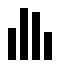
\includegraphics[scale=0.14]{homepage.png} \url{https://nimahejazi.org}

\vspace{2mm}
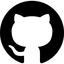
\includegraphics[scale=0.11]{github-icon.png}
  \url{https://github.com/nhejazi}

\vspace{2mm}

\includegraphics[scale=0.14]{twitter-icon.png}
  \url{https://twitter.com/nshejazi}

\end{frame}

%%%%%%%%%%%%%%%%%%%%%%%%%%%%%%%%%%%%%%%%%%%%%%%%%%%%%%%%%%%%%%%%%%%%%%%%%%%%%%%%

%\appendix
%\begin{frame}[standout]
  %Appendix
%\end{frame}

%%%%%%%%%%%%%%%%%%%%%%%%%%%%%%%%%%%%%%%%%%%%%%%%%%%%%%%%%%%%%%%%%%%%%%%%%%%%%%%%

%\begin{frame}[c]{Nonparametric Conditional Density Estimation}

%\begin{center}
%\begin{itemize}
  %\itemsep8pt
  %\item To compute the auxiliary covariate $H(a,w)$, we need to estimate
    %conditional densities $g(A \mid W)$ and $g(A - \delta \mid W)$.
  %\item There is a rich literature on density estimation, we follow the approach
    %proposed in \cite{diaz2011super}.
  %\item To build a conditional density estimator, consider
    %\begin{equation*}
      %g_{n, \alpha}(a \mid W) = \frac{\pr (A \in [\alpha_{t-1}, \alpha_t)
        %\mid W)}{\alpha_t - \alpha_{t-1}},
    %\end{equation*}
    %for $\alpha_{t-1} \leq a < \alpha_t$.
    %\vspace{0.5em}
    %\begin{itemize}
      %\itemsep4pt
      %\item This is a classification problem, where we estimate the probability
        %that a value of $A$ falls in a bin $[\alpha_{t-1}, \alpha_t)$.
      %\item The choice of the tuning parameter $t$ corresponds roughly to the
        %choice of bandwidth in classical kernel density estimation.
    %\end{itemize}
%\end{itemize}
%\end{center}

%\note{
%}

%\end{frame}

%%%%%%%%%%%%%%%%%%%%%%%%%%%%%%%%%%%%%%%%%%%%%%%%%%%%%%%%%%%%%%%%%%%%%%%%%%%%%%%%

\end{document}
